\documentclass[a4paper,11pt]{article}
\usepackage[left=2.5cm,right=2.5cm,top=2.5cm]{geometry}
\usepackage[czech,slovak,english]{babel}
\usepackage[utf8]{inputenc}
\usepackage{url}
\usepackage{graphicx}
\usepackage{picture}

\usepackage{listings}
\usepackage[toc,page,header]{appendix}
\RequirePackage{titletoc}

\addto\captionsenglish{\renewcommand{\figurename}{Obr.}}

\begin{document}

\section{Enumeration Sort}
Enumeration sort je je radiaci algoritmus, ktorý vzájomným porovnávaním všetkých prvkov nájde ich zoradenú postupnosť. V tomto prípade sa jedná o variantu pracujúcu nad lineárnym poľom N procesorov doplnených o spoločnú zbernicu a schopných preniesť jednu hodnotu v každom kroku. Počet procesorov odpovedá počtu radených prvkov.

Ak na vstupe máme radu $X=(x_1, x_2, ..., x_n)$, potom každý procesor $i \in <1,N>$ pozostáva zo 4 registrov, ktoré obsahujú:
\begin{itemize}
\item $X_i$ prvok $x_i$ zo vstupnej rady
\item $Y_i$ postupne prvky $x_1$..$x_n$
\item $C_i$ koľkokrát platilo $X_i > Y_i$
\item $Z_i$ zoradený prvok $Y_i$
\end{itemize}

\begin{figure}[!htb]
\centering
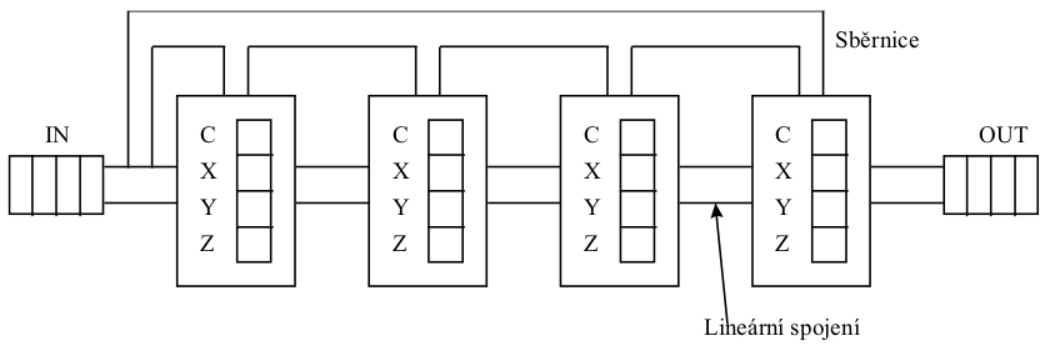
\includegraphics[width=\textwidth]{es.png}
\caption{Architektúra Enumeration Sort (Zdroj: Slidy PRL)}
\end{figure}

\subsection{Algoritmus}
\begin{enumerate}
\item Všetky registre C sa nastavia na hodnotu 1
\item 2n-krát opakuj ($ 1 \leq k \leq 2n$):
\begin{itemize}
\item Ak nie je vstup vyčerpaný, vstupný prvok $x_i$ sa vloží prostredníctvom zbernice do $X_i$ a lineárnym spojením sa obsah všetkých registrov $Y$ posunie doprava a do $Y_1$ sa vloží prvok $x_i$
\item Každý procesor $p$ s neprázdnymi registrami $X_p$ a $Y_p$ ich porovná a v prípade, ak $X_p > Y_p$ inkrementuje register $C_p$
\item Ak $k > n$, procesor $P_{k-n}$ pošle obsah svojho registru $X$ procesoru $P_{C_{k-1}}$, ktorý si túto hodnotu uloží do registru $Z$
\end{itemize}
\item V nasledujúcich n cykloch procesory posúvajú obsah svojich registrov Z doprava a procesor $P_n$ produkuje zoradenú postupnosť.
\end{enumerate}


\begin{figure}[!htb]
\centering
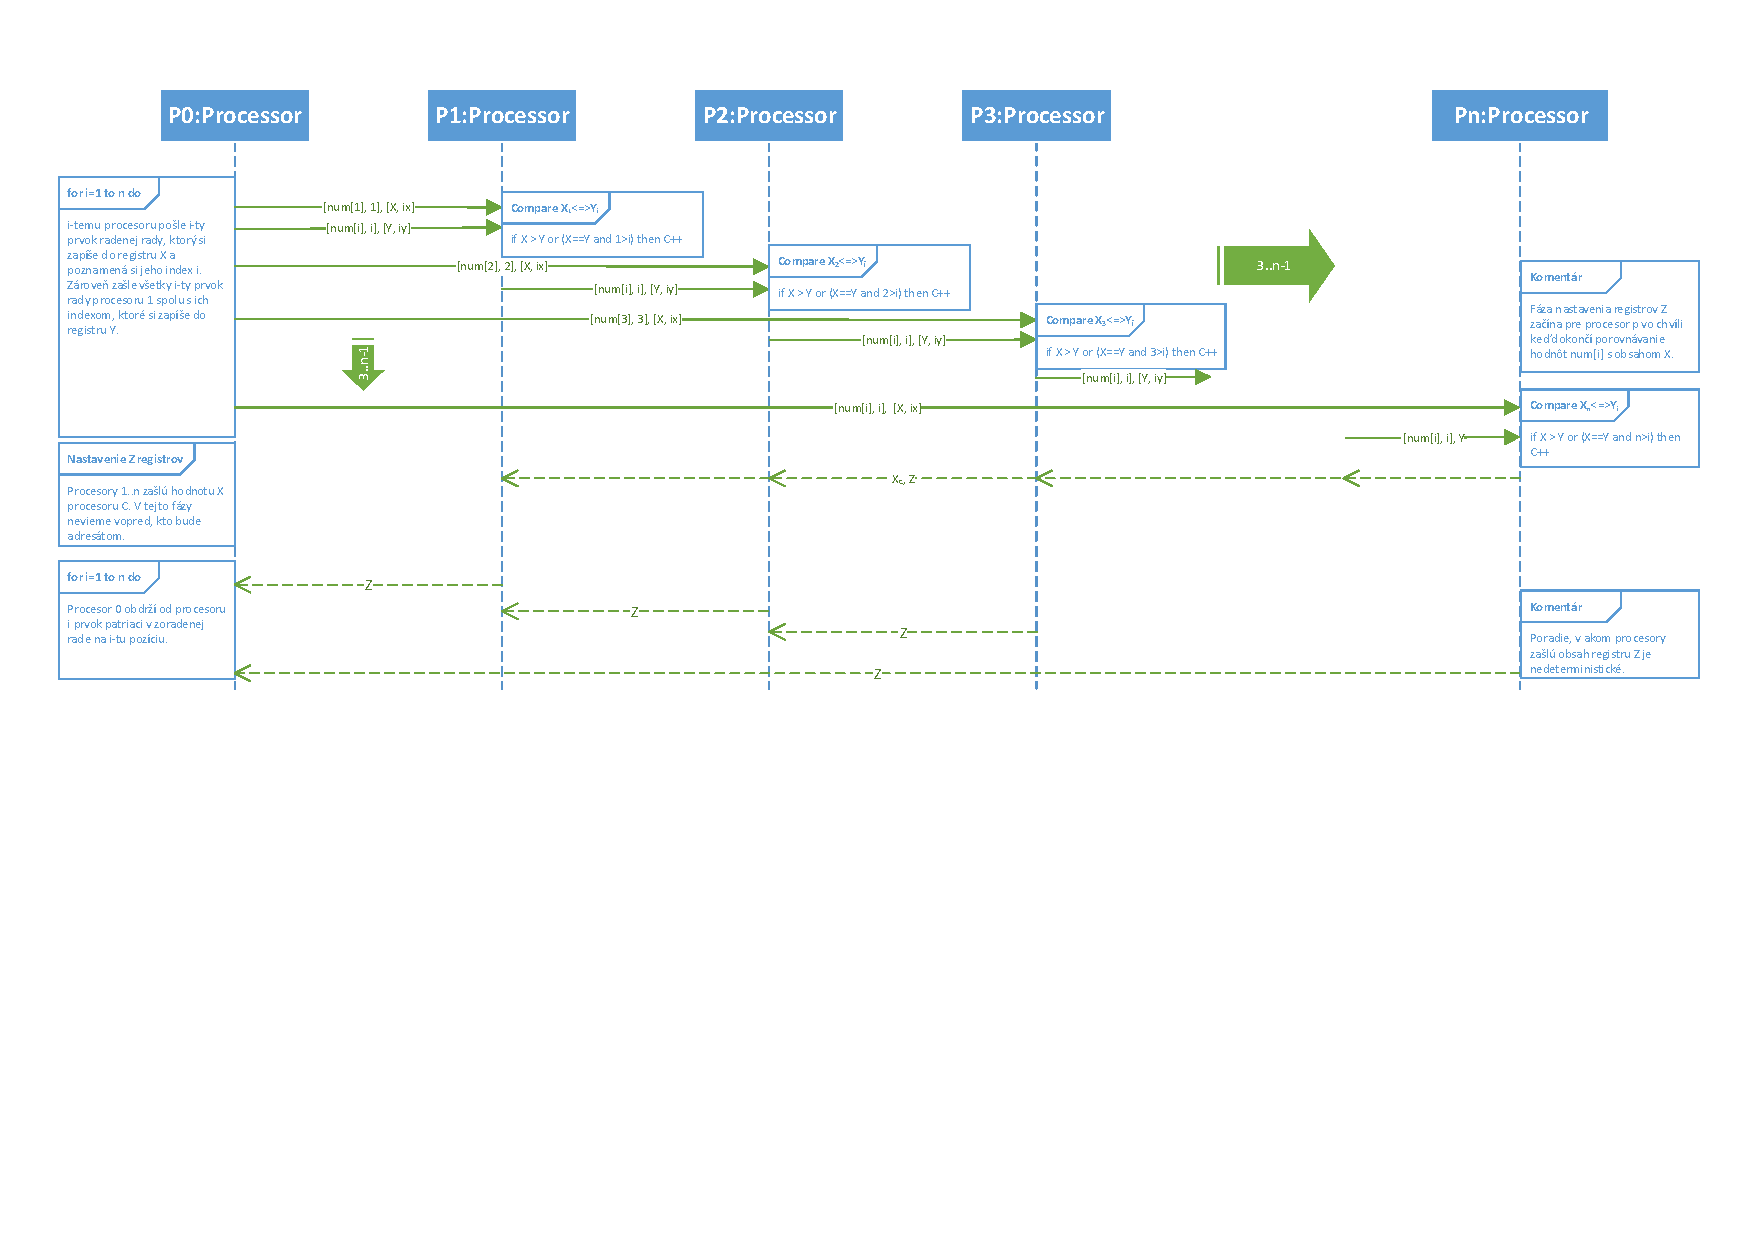
\includegraphics[width=\textwidth]{sequence.pdf}
\caption{Sekvenčný diagram}
\end{figure}

\begin{figure}[!htb]
\centering
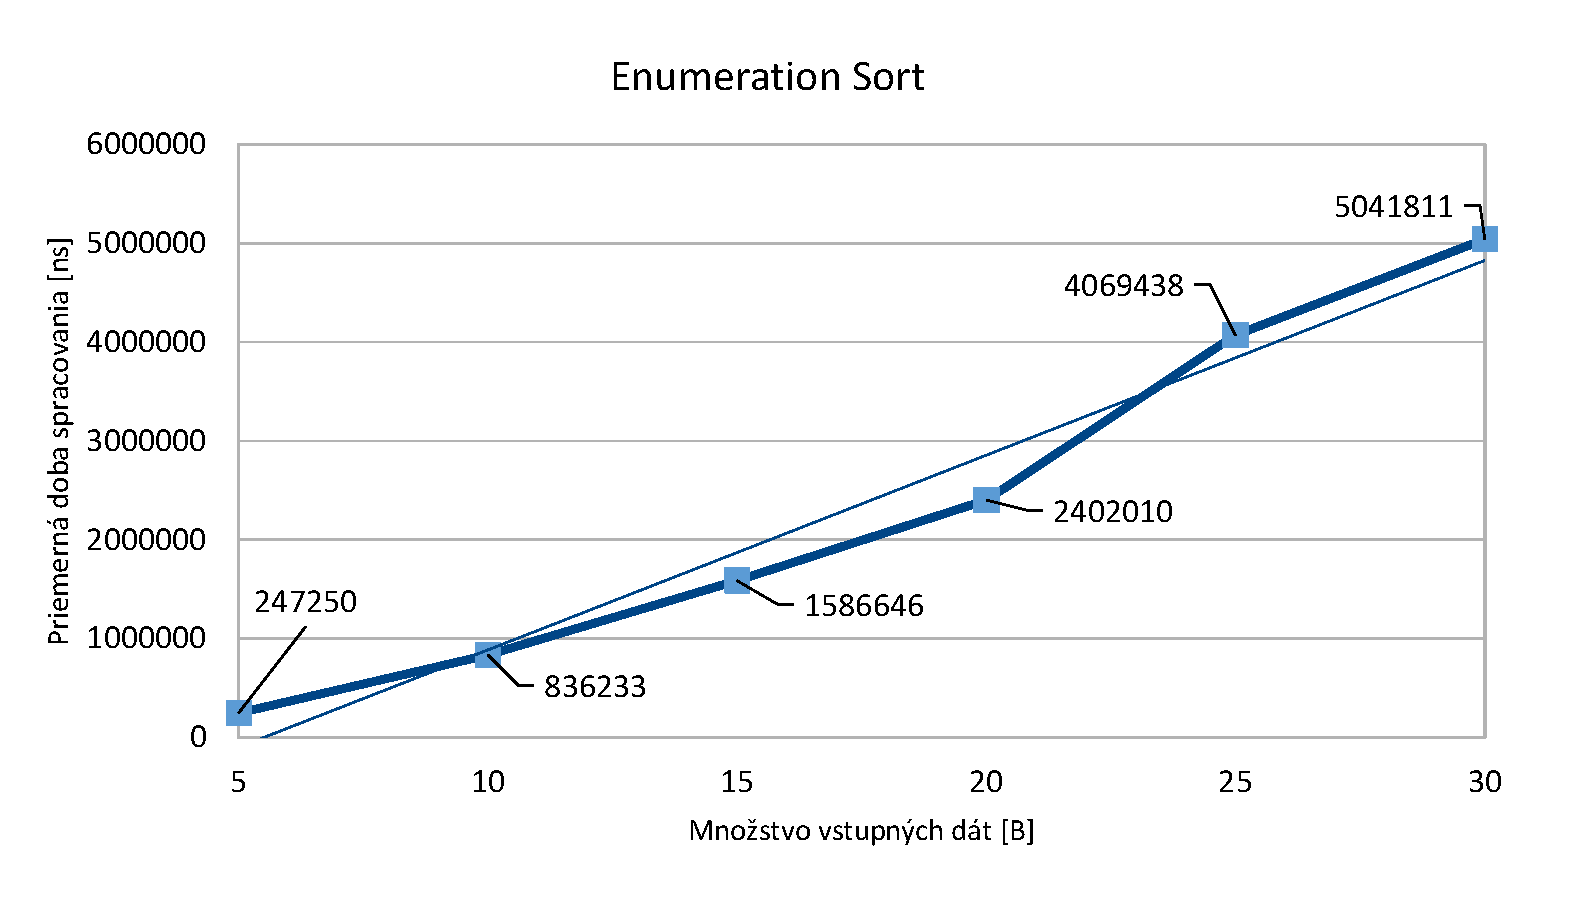
\includegraphics[width=\textwidth]{stats.pdf}
\caption{Namerané časy}
\end{figure}

\end{document}
